\documentclass[12pt,a4paper]{article}
\usepackage[utf8]{inputenc}
\usepackage[vietnamese]{babel}
\usepackage{geometry}
\usepackage{fancyhdr}
\usepackage{listings}
\usepackage{titlesec}
\usepackage{tocloft}
\usepackage{graphicx}
\usepackage{array}
\usepackage{longtable}
\usepackage{booktabs}
\usepackage{xcolor}
\usepackage[most]{tcolorbox}
\usepackage{enumitem}
\usepackage{amsmath, amssymb}
\usepackage{hyperref}
\usepackage{times}
\usepackage{algorithm}
\usepackage{algorithmic}

% Page setup
\geometry{margin=1in}
\pagestyle{fancy}
\fancyhf{}
\fancyhead[L]{Tổ hợp và Lý thuyết Đồ thị}
\fancyhead[R]{PNDK - Final Report}
\fancyfoot[C]{\thepage}

% Color definitions
\definecolor{titleblue}{RGB}{44,90,160}
\definecolor{lightblue}{RGB}{230,243,255}
\definecolor{releasegreen}{RGB}{46,125,50}
\definecolor{sprintblue}{RGB}{33,150,243}

% Title formatting
\titleformat{\section}{\large\bfseries\color{titleblue}}{\thesection}{1em}{}
\titleformat{\subsection}{\normalsize\bfseries}{\thesubsection}{1em}{}
\titleformat{\subsubsection}{\small\bfseries}{\thesubsubsection}{1em}{}

% Khung đề
\newtcolorbox{problembox}{
    title=\textbf{Đề bài}, 
    colback=white,         
    colframe=black,        
    fonttitle=\bfseries,   
    boxsep=5pt,           
    left skip=0mm,         
    right skip=0mm,        
    width=\textwidth,              
    enlarge top by=1ex,    
    enlarge bottom by=1ex, 
    before skip=1em,       
    after skip=1em         
}
% Hyperref setup
\hypersetup{
    colorlinks=true,
    linkcolor=titleblue,
    filecolor=magenta,      
    urlcolor=cyan,
    pdftitle={},
    pdfauthor={}
}

\begin{document}

% Title Page
\begin{titlepage}
    \centering
    
    % Logo
    
\includegraphics[width=0.3\textwidth]{assets/logo_umt_value.png}
    \vspace{1cm}
    
    {\LARGE\bfseries TỔ HỢP VÀ LÝ THUYẾT ĐỒ THỊ\par}
    \vspace{0.5cm}
    
    {\Large Học kỳ: Mùa hè 2025\par}
    \vspace{1.5cm}
    
    {\large Sinh viên thực hiện:\par}
    \vspace{0.5cm}
    \begin{tabular}{ll}
        2201700147 & - Phan Nguyễn Duy Kha \\
    \end{tabular}
    
    \vspace{1cm}
    {\large Giảng viên hướng dẫn: \textbf{Nguyễn Quản Bá Hồng}\par}
    
    \vfill
    
    % Release Plan Box
    \colorbox{lightblue}{%
        \begin{minipage}{0.8\textwidth}
            \centering
            \vspace{1cm}
            {\Huge\bfseries FINAL PROJECT\par}
            \vspace{0.5cm}
            {\large Đồ án cuối kỳ môn học\par}
            \vspace{1cm}
        \end{minipage}
    }
    
    \vfill
    
    {\large Khoa Công nghệ\par}
    {\large Trường Đại học Quản lý và Công nghệ TP.HCM\par}
    
\end{titlepage}

% Revision History Page
\newpage
\thispagestyle{empty}

\begin{center}
{\Huge\bfseries LỊCH SỬ SỬA ĐỔI\par}
\end{center}

\renewcommand{\arraystretch}{1.5}
\begin{center}
\begin{longtable}{|p{3cm}|p{8cm}|p{3cm}|}
\hline
\textbf{Ngày} & \textbf{Mô tả} & \textbf{Tác giả} \\
\hline
\endhead
10/07/2025 & Khởi tạo file báo cáo & Duy Kha\\
\hline
14/07/2025 & Cập nhật Project 5 & Duy Kha\\
\hline
\end{longtable}
\end{center}

% Table of Contents
\newpage
\tableofcontents

% Main Content
\newpage

\section{Tổng quan các Project}

\subsection{Project 1: Quy Nạp Toán Học và Quan Hệ Truy Hồi}

\subsection{Project 2: Đếm, Xác Suất, Banh và Hộp}

\subsection{Project: Phân Hoạch Số Nguyên}

\subsection{Project 4: Các Bài Toán Duyệt Đồ Thị và Cây}

\subsection{Project 5: Các Bài Toán Tìm Đường Đi Ngắn Nhất Trên Đồ Thị}

\newpage

\section{Project 3:  Integer Partition – Đồ Án: Phân Hoạch Số Nguyên}

\subsection{Bài toán 1: Biểu đồ Ferrers and biểu đồ Ferrers chuyển vị}

\begin{problembox}
Nhập $n, k \in \mathbb{N}$. Viết chương trình C/C++, Python để in ra $p_k(n)$ biểu đồ Ferrers $F$ \& biểu đồ Ferrers chuyển vị $F^\top$ cho mỗi phân hoạch $\lambda = (\lambda_1, \lambda_2, \ldots, \lambda_k) \in (\mathbb{N}^*)^k$ có định dạng các dấu chấm được biểu diễn bởi dấu *.

\end{problembox}

\textbf{Phân tích đề bài:}


\begin{itemize}[label=\textbullet]
    \item \textbf{Input:} Hai số nguyên dương n và k
    \item \textbf{Yêu cầu:} Tìm tất cả các phân hoạch của n thành đúng k phần
    \item \textbf{Output:} Với mỗi phân hoạch, in biểu đồ Ferrers và biểu đồ Ferrers chuyển vị
    \item \textbf{Định dạng:} Sử dụng dấu * để biểu diễn các phần tử trong biểu đồ
\end{itemize}

\textbf{Kiến thức nền tảng:}
\vspace{0.2cm}

\textbf{Phân hoạch số nguyên (Integer Partition):} 
\begin{itemize}[label=\textbullet]
    \item Là cách viết số nguyên dương n thành tổng các số nguyên dương
    \item Ví dụ: 5 = 5 = 4+1 = 3+2 = 3+1+1 = 2+2+1 = 2+1+1+1 = 1+1+1+1+1
\end{itemize}


\textbf{Phân hoạch thành k phần (pk(n)):} 
\begin{itemize}[label=\textbullet]
    \item Là các phân hoạch có đúng k số hạng
    \item Ký hiệu: $\lambda = (\lambda_1, \lambda_2, \ldots, \lambda_k)$ với $\lambda_1 \geq \lambda_2 \geq \ldots \geq \lambda_k \geq 1$ và $\sum_{i=1}^{k} \lambda_i = n$
\end{itemize}

\textbf{Biểu đồ Ferrers:} 
\begin{itemize}[label=\textbullet]
    \item Biểu diễn hình học của phân hoạch bằng các hàng dấu *
    \item Hàng thứ i có $\lambda_i$ dấu *
    \item Các hàng sắp xếp từ trên xuống theo thứ tự không tăng
\end{itemize}

\textbf{Biểu đồ Ferrers chuyển vị ($F^T$):} 
\begin{itemize}[label=\textbullet]
    \item Là biểu đồ Ferrers của phân hoạch liên hợp
    \item Được tạo bằng cách hoán đổi hàng và cột của biểu đồ gốc
    \item Phần tử thứ j trong phân hoạch chuyển vị = số dấu * ở cột thứ j của biểu đồ gốc
\end{itemize}

\textbf{Công thức và tính chất:} 
\begin{itemize}[label=\textbullet]
    \item \textbf{Điều kiện phân hoạch:}
$$\lambda = (\lambda_1, \lambda_2, \ldots, \lambda_k) \text{ với } \lambda_1 \geq \lambda_2 \geq \ldots \geq \lambda_k \geq 1$$
$$\sum_{i=1}^{k} \lambda_i = n$$
    \item \textbf{Giới hạn giá trị:} Nếu $\lambda = (\lambda_1, \lambda_2, \ldots, \lambda_k)$ thì $\lambda^T = (\mu_1, \mu_2, \ldots, \mu_m)$ với:
$$\mu_j = |\{i : \lambda_i \geq j\}|$$
\end{itemize}

\textbf{Ý tưởng thuật toán:} 
\paragraph{Bước 1: Sinh phân hoạch $p_k(n)$}
\begin{enumerate}
    \item Sử dụng đệ quy để sinh tất cả các phân hoạch
    \item Đảm bảo thứ tự không tăng: $\lambda_1 \geq \lambda_2 \geq \ldots \geq \lambda_k$
    \item Giới hạn giá trị của phần tử đầu tiên để đảm bảo tồn tại phân hoạch
\end{enumerate}

\paragraph{Bước 2: Vẽ biểu đồ Ferrers}
\begin{enumerate}
    \item Với mỗi phần $\lambda_i$, in ra $\lambda_i$ dấu *
    \item Xuống dòng sau mỗi hàng
\end{enumerate}

\paragraph{Bước 3: Tìm và vẽ biểu đồ chuyển vị}
\begin{enumerate}
    \item Đếm số dấu * ở mỗi cột của biểu đồ gốc
    \item Tạo phân hoạch mới từ các giá trị đếm được
    \item Vẽ biểu đồ Ferrers cho phân hoạch mới
\end{enumerate}

\textbf{Cài đặt Python:}
\begin{itemize}[label=\textbullet]
   \item File tổng hợp: \texttt{.\textbackslash code\textbackslash Project\_3\textbackslash BT1\textbackslash ferrers\_diagrams.py}
\end{itemize}

\textbf{Cài đặt C++:}
\begin{itemize}[label=\textbullet]
   \item File tổng hợp: \texttt{.\textbackslash code\textbackslash Project\_3\textbackslash BT1\textbackslash ferrers\_diagrams.cpp}
\end{itemize}
\newpage

\subsection{Bài toán 2:}

\begin{problembox}
Nhập $n, k \in \mathbb{N}$. Đếm số phân hoạch của $n$ sao cho phần tử lớn nhất là $k$. So sánh $p_k(n)$ \& $p_{\max}(n, k)$.

\end{problembox}

\textbf{Phân tích đề bài:}


\begin{itemize}[label=\textbullet]
    \item \textbf{Input:} Hai số nguyên dương n và k
    \item \textbf{Yêu cầu:}
    \item Tính $p_{\max}(n, k)$ - số phân hoạch của n sao cho phần tử lớn nhất là k
    \item So sánh $p_k(n)$ (số phân hoạch thành đúng k phần) và $p_{\max}(n, k)$

\end{itemize}

- \textbf{Ví dụ:}
        
            
- n = 5, k = 3: Các phân hoạch có phần tử lớn nhất là 3:
                
                    
- (3, 2)
                    
- (3, 1, 1)
                
                $\Rightarrow p_{\max}(5, 3) = 2$
            
- $p_3(5)$ (phân hoạch thành đúng 3 phần): (3, 2), (3, 1, 1), (2, 2, 1)
                $\Rightarrow p_3(5) = 3$

\vspace{0.5cm}
\textbf{Kiến thức nền tảng:}

\paragraph{Phân hoạch $p_k(n)$:}
Là số cách viết n thành tổng các số nguyên dương không tăng với đúng k số hạng.

\paragraph{Phân hoạch $p_{\max}(n, k)$:}
Là số cách viết n thành tổng các số nguyên dương không tăng sao cho phần tử lớn nhất là k.

\paragraph{Liên hệ giữa $p_k(n)$ và $p_{\max}(n, k)$:}
[label=$\bullet$]
    
- $p_k(n)$ và $p_{\max}(n, k)$ là hai khái niệm khác nhau
    
- $p_k(n)$: cố định số phần = k
    
- $p_{\max}(n, k)$: cố định phần tử lớn nhất = k


\subsubsection*{Ý tưởng thuật toán:}

\paragraph{Tính $p_{\max}(n, k)$:}
\begin{enumerate}
    \item Sinh tất cả phân hoạch của n
    \item Lọc ra các phân hoạch có phần tử lớn nhất = k
    \item Đếm số lượng phân hoạch thỏa mãn
\end{enumerate}

\paragraph{Tính $p_k(n)$:}
\begin{enumerate}
    \item Sinh tất cả phân hoạch của n thành đúng k phần
    \item Đếm số lượng phân hoạch
\end{enumerate}

\textbf{Cài đặt Python:}
\begin{itemize}[label=\textbullet]
   \item File tổng hợp: \texttt{.\textbackslash code\textbackslash Project\_3\textbackslash BT2\textbackslash partition\_comparison.py}
\end{itemize}

\textbf{Cài đặt C++:}
\begin{itemize}[label=\textbullet]
   \item File tổng hợp: \texttt{.\textbackslash code\textbackslash Project\_3\textbackslash BT2\textbackslash partition\_comparison.cpp}
\end{itemize}

\subsection{Bài toán 3:}

\begin{problembox}
Nhập $n, k \in \mathbb{N}$.
\begin{enumerate}
    \item[(a)] Đếm số phân hoạch tự liên hợp của $n$ có $k$ phần, ký hiệu $p_k^{\text{self-conj}}(n)$, rồi in ra các phân hoạch đó.
    \item[(b)] Đếm số phân hoạch của $n$ có lẻ phần, rồi so sánh với $p_k^{\text{self-conj}}(n)$.
    \item[(c)] Thiết lập công thức truy hồi cho $p_k^{\text{self-conj}}(n)$, rồi implement bằng:
    \begin{enumerate}
        \item[(i)] đệ quy,
        \item[(ii)] quy hoạch động.
    \end{enumerate}
\end{enumerate}


\textbf{Phân tích đề bài:}


\begin{itemize}[label=\textbullet]
    \item \textbf{Input:} Hai số nguyên dương n và k
    \item \textbf{Yêu cầu:}
    \item Tính $p_{\max}(n, k)$ - số phân hoạch của n sao cho phần tử lớn nhất là k
    \item So sánh $p_k(n)$ (số phân hoạch thành đúng k phần) và $p_{\max}(n, k)$

\end{itemize}

\end{problembox}

\section{Project 4: Các Bài Toán Duyệt Đồ Thị và Cây}

\subsection{Bài toán 4: Chuyển đổi giữa các dạng biểu diễn đồ thị và cây}

\begin{problembox}
    \textbf{Viết chương trình C/C++, Python chuyển đổi giữa 4 dạng biểu diễn: adjacency matrix, adjacency list, extended adjacency list, adjacency map cho 3 đồ thị: đơn đồ thị, đa đồ thị, đồ thị tổng quát; \& 3 dạng biểu diễn: array of parents, first-child next-sibling, graph-based representation of trees của cây.} 
    
    Sẽ có $3 \times A_4^3 + A_2^3 = 36 + 6 = 42$ converter programs.

\end{problembox}

\textbf{Phân tích bài toán:} Bài toán yêu cầu implement tổng cộng 42 converter functions, được chia thành:

\begin{itemize}
    \item \textbf{Đồ thị:} $3 \times 4 \times 3 = 36$ converters (3 loại đồ thị × 4 dạng biểu diễn × 3 chuyển đổi mỗi dạng)
    \item \textbf{Cây:} $3 \times 2 = 6$ converters (3 dạng biểu diễn × 2 chuyển đổi mỗi dạng)
\end{itemize}

\textbf{Cài đặt Python:}
\begin{itemize}[label=\textbullet]
   \item File: \texttt{.\textbackslash code\textbackslash Project\_4\textbackslash BT4\textbackslash simple\_graph\textbackslash simple\_graph.py}
   \item  File: \texttt{.\textbackslash code\textbackslash Project\_4\textbackslash BT4\textbackslash multi\_graph\textbackslash multi\_graph.py}
   \item  File: \texttt{.\textbackslash code\textbackslash Project\_4\textbackslash BT4\textbackslash general\_graph\textbackslash general\_graph.py}
   \item  File: \texttt{.\textbackslash code\textbackslash Project\_4\textbackslash BT4\textbackslash \textbackslash tree\textbackslash tree.py}
\end{itemize}

\textbf{Cài đặt C++:}
\begin{itemize}[label=\textbullet]
   \item File: \texttt{.\textbackslash code\textbackslash Project\_4\textbackslash BT4\textbackslash simple\_graph\textbackslash simple\_graphy.cpp }
   \item File: \texttt{.\textbackslash code\textbackslash Project\_4\textbackslash BT4\textbackslash multi\_graph\textbackslash multi\_graph.cpp }
   \item File: \texttt{.\textbackslash code\textbackslash Project\_4\textbackslash BT4\textbackslash general\_graph\textbackslash general\_graph.cpp }
   \item File: \texttt{.\textbackslash code\textbackslash Project\_4\textbackslash BT4\textbackslash tree\textbackslash tree.cpp }
\end{itemize}
\newpage
\subsubsection{Simple Graph (Đơn đồ thị) - 12 Converters}

\textbf{Định nghĩa:} Simple Graph $G = (V, E)$ là đồ thị không có cạnh song song và không có khuyên (self-loops).
\vspace{0.5cm}

\textbf{4 dạng biểu diễn:}
\begin{itemize}[label=\textbullet]
    \item 1. Adjacency Matrix (Ma trận kề)
    \item 2. Adjacency List (Danh sách kề)
    \item 3. Extended Adjacency List
    \item 4. Adjacency Map
\end{itemize}

\textbf{Converter 1: Matrix $\rightarrow$ List}

\textbf{Ý tưởng chính:} Duyệt upper triangle của ma trận đối xứng để tránh xử lý duplicate edges.

\textbf{Thuật toán:}
\begin{enumerate}
    \item Khởi tạo $n$ danh sách rỗng cho adjacency list
    \item Chỉ duyệt các vị trí $(i,j)$ với $i \leq j$ (upper triangle)
    \item Nếu $matrix[i][j] = 1$:
    \begin{itemize}
        \item Nếu $i = j$: thêm $j$ vào $adj\_list[i]$ (self-loop)
        \item Nếu $i \neq j$: thêm $j$ vào $adj\_list[i]$ và $i$ vào $adj\_list[j]$ (undirected)
    \end{itemize}
\end{enumerate}
\vspace{0.5cm}

\textbf{Converter 2: Matrix $\rightarrow$ Extended List}

\textbf{Ý tưởng chính:} Tương tự Matrix $\rightarrow$ List nhưng tạo Edge objects thay vì chỉ lưu đỉnh.

\textbf{Thuật toán:}
\begin{enumerate}
    \item Duyệt upper triangle của ma trận
    \item Với mỗi cạnh $(i,j)$ tìm được:
    \begin{itemize}
        \item Tạo $Edge(i,j)$ và thêm vào $outgoing[i]$, $incoming[j]$
        \item Nếu $i \neq j$: tạo $Edge(j,i)$ và thêm vào $outgoing[j]$, $incoming[i]$
        \item Thêm cả 2 edges vào $all\_edges$
    \end{itemize}
\end{enumerate}
\vspace{0.5cm}

\textbf{Converter 3: Matrix $\rightarrow$ Map}

\textbf{Ý tưởng chính:} Duyệt toàn bộ ma trận và thêm neighbors vào hash set.

\textbf{Thuật toán:}
\begin{enumerate}
    \item Khởi tạo $n$ hash sets rỗng
    \item Duyệt toàn bộ ma trận $(i,j)$ với $0 \leq i,j < n$
    \item Nếu $matrix[i][j] = 1$: thêm $j$ vào $adj\_map[i]$
\end{enumerate}
\vspace{0.5cm}

\textbf{Converter 4: List $\rightarrow$ Matrix}

\textbf{Ý tưởng chính:} Duyệt adjacency list và đánh dấu các vị trí tương ứng trong ma trận.

\textbf{Thuật toán:}
\begin{enumerate}
    \item Khởi tạo ma trận $n \times n$ toàn $0$
    \item Với mỗi đỉnh $u = 0, 1, \ldots, n-1$:
    \item Với mỗi neighbor $v \in adj\_list[u]$: đặt $matrix[u][v] = 1$
\end{enumerate}
\vspace{0.5cm}

\textbf{Converter 5: List $\rightarrow$ Extended List}

\textbf{Ý tưởng chính:} Tránh tạo duplicate Edge objects bằng canonical form technique.

\textbf{Thuật toán:}
\begin{enumerate}
    \item Khởi tạo $processed\_edges = \emptyset$ (hash set)
    \item Với mỗi đỉnh $u$ và neighbor $v \in adj\_list[u]$:
    \begin{itemize}
        \item Tính $edge\_key = (\min(u,v), \max(u,v))$
        \item Nếu $edge\_key \notin processed\_edges$:
        \begin{itemize}
            \item Thêm $edge\_key$ vào $processed\_edges$
            \item Tạo $Edge(u,v)$ và $Edge(v,u)$
            \item Cập nhật các cấu trúc dữ liệu
        \end{itemize}
    \end{itemize}
\end{enumerate}
\vspace{0.5cm}

\textbf{Converter 6: List $\rightarrow$ Map}

\textbf{Ý tưởng chính:} Chuyển đổi trực tiếp từ list sang set cho mỗi đỉnh.

\textbf{Thuật toán:}
\begin{enumerate}
    \item Với mỗi đỉnh $u = 0, 1, \ldots, n-1$:
    \item Chuyển $adj\_list[u]$ (list) thành $adj\_map[u]$ (set)
\end{enumerate}
\vspace{0.5cm}

\textbf{Converter 7: Extended List $\rightarrow$ Matrix}

\textbf{Ý tưởng chính:} Đơn giản nhất - duyệt tất cả edges và đánh dấu ma trận.

\textbf{Thuật toán:}
\begin{enumerate}
    \item Khởi tạo ma trận $n \times n$ toàn $0$
    \item Với mỗi $edge \in all\_edges$:
    \item Đặt $matrix[edge.source][edge.target] = 1$
\end{enumerate}
\vspace{0.5cm}

\textbf{Converter 8: Extended List $\rightarrow$ List}

\textbf{Ý tưởng chính:} Trích xuất target vertices từ outgoing edges.

\textbf{Thuật toán:}
\begin{enumerate}
    \item Với mỗi đỉnh $u = 0, 1, \ldots, n-1$:
    \item Với mỗi $edge \in outgoing[u]$:
    \item Thêm $edge.target$ vào $adj\_list[u]$ (nếu chưa có)
\end{enumerate}
\vspace{0.5cm}

\textbf{Converter 9: Extended List $\rightarrow$ Map}

\textbf{Ý tưởng chính:} Tương tự converter 8 nhưng sử dụng set thay vì list.

\textbf{Thuật toán:}
\begin{enumerate}
    \item Với mỗi đỉnh $u = 0, 1, \ldots, n-1$:
    \item Với mỗi $edge \in outgoing[u]$:
    \item Thêm $edge.target$ vào $adj\_map[u]$ (set tự động loại duplicate)
\end{enumerate}
\vspace{0.5cm}

\textbf{Converter 10: Map $\rightarrow$ Matrix}

\textbf{Ý tưởng chính:} Duyệt hash sets và đánh dấu ma trận.

\textbf{Thuật toán:}
\begin{enumerate}
    \item Khởi tạo ma trận $n \times n$ toàn $0$
    \item Với mỗi đỉnh $u = 0, 1, \ldots, n-1$:
    \item Với mỗi $v \in adj\_map[u]$: đặt $matrix[u][v] = 1$
\end{enumerate}
\vspace{0.5cm}

\textbf{Converter 11: Map $\rightarrow$ List}

\textbf{Ý tưởng chính:} Chuyển đổi trực tiếp từ set sang list cho mỗi đỉnh.

\textbf{Thuật toán:}
\begin{enumerate}
    \item Với mỗi đỉnh $u = 0, 1, \ldots, n-1$:
    \item Chuyển $adj\_map[u]$ (set) thành $adj\_list[u]$ (list)
\end{enumerate}
\vspace{0.5cm}

\textbf{Converter 12: Map $\rightarrow$ Extended List}

\textbf{Ý tưởng chính:} Chuyển đổi gián tiếp qua List để tái sử dụng algorithm đã có.

\textbf{Thuật toán:}
\begin{enumerate}
    \item Gọi $list\_graph = $ Map $\rightarrow$ List$(map\_graph)$
    \item Gọi $ext\_graph = $ List $\rightarrow$ Extended List$(list\_graph)$
    \item Trả về $ext\_graph$
\end{enumerate}

\subsubsection{Multigraph (Đa đồ thị) - 12 Converters}

\textbf{Định nghĩa:} Multigraph $G = (V, E)$ là đồ thị cho phép có nhiều cạnh song song giữa hai đỉnh (parallel edges) nhưng không có khuyên (self-loops).
\vspace{0.5cm}

\textbf{4 dạng biểu diễn:}
\begin{itemize}[label=\textbullet]
    \item 1. Adjacency Matrix (Ma trận kề): $matrix[i][j] \in \{0, 1, 2, 3, \ldots\}$ - số cạnh giữa đỉnh $i$ và $j$
    \item 2. Adjacency List (Danh sách kề): cho phép entries trùng lặp
    \item 3. Extended Adjacency List: nhiều Edge objects cho cùng một cặp đỉnh
    \item 4. Adjacency Map: $adj\_map[u][v] = count$ - số cạnh từ $u$ đến $v$
\end{itemize}

\textbf{Converter 1: Matrix $\rightarrow$ List}

\textbf{Ý tưởng chính:} Duyệt upper triangle và thêm multiple entries cho parallel edges.

\textbf{Thuật toán:}
\begin{enumerate}
    \item Khởi tạo $n$ danh sách rỗng cho adjacency list
    \item Chỉ duyệt các vị trí $(i,j)$ với $i \leq j$ (upper triangle)
    \item Nếu $matrix[i][j] = count > 0$:
    \begin{itemize}
        \item Nếu $i = j$: thêm $j$ vào $adj\_list[i]$ đúng $count$ lần (self-loop)
        \item Nếu $i \neq j$: thêm $j$ vào $adj\_list[i]$ và $i$ vào $adj\_list[j]$ mỗi cái $count$ lần
    \end{itemize}
\end{enumerate}

\vspace{0.5cm}

\textbf{Converter 2: List $\rightarrow$ Matrix}

\textbf{Ý tưởng chính:} Đếm frequency của mỗi neighbor thay vì chỉ đánh dấu 0/1.

\textbf{Thuật toán:}
\begin{enumerate}
    \item Khởi tạo ma trận $n \times n$ toàn $0$
    \item Với mỗi đỉnh $u = 0, 1, \ldots, n-1$:
    \begin{itemize}
        \item Tạo $neighbor\_count = \emptyset$ (hash map)
        \item Với mỗi $v \in adj\_list[u]$: tăng $neighbor\_count[v]$
        \item Với mỗi $(v, count) \in neighbor\_count$: đặt $matrix[u][v] = count$
    \end{itemize}
\end{enumerate}

\vspace{0.5cm}

\textbf{Converter 3: Matrix $\rightarrow$ Extended List}

\textbf{Ý tưởng chính:} Tạo multiple Edge objects cho parallel edges, mỗi edge có unique ID.

\textbf{Thuật toán:}
\begin{enumerate}
    \item Duyệt upper triangle của ma trận
    \item Với mỗi cạnh $(i,j)$ có $matrix[i][j] = count > 0$:
    \begin{itemize}
        \item Lặp $count$ lần:
        \begin{itemize}
            \item Tạo $Edge(i,j, weight, unique\_id)$
            \item Thêm vào $outgoing[i]$, $incoming[j]$, $all\_edges$
            \item Nếu $i \neq j$: tạo $Edge(j,i)$ tương tự
        \end{itemize}
    \end{itemize}
\end{enumerate}

\vspace{0.5cm}

\textbf{Converter 4: Extended List $\rightarrow$ Matrix}

\textbf{Ý tưởng chính:} Đếm frequency của mỗi $(source, target)$ pair từ $all\_edges$.

\textbf{Thuật toán:}
\begin{enumerate}
    \item Khởi tạo ma trận $n \times n$ toàn $0$
    \item Tạo $edge\_count = \emptyset$ (hash map)
    \item Với mỗi $edge \in all\_edges$: tăng $edge\_count[(edge.source, edge.target)]$
    \item Với mỗi $((u,v), count) \in edge\_count$: đặt $matrix[u][v] = count$
\end{enumerate}

\vspace{0.5cm}

\textbf{Converter 5: List $\rightarrow$ Extended List}

\textbf{Ý tưởng chính:} Sử dụng canonical form để tránh duplicate và xử lý đúng undirected edges.

\textbf{Thuật toán:}
\begin{enumerate}
    \item Tạo $edge\_count = \emptyset$ (hash map)
    \item Với mỗi đỉnh $u$ và neighbor $v \in adj\_list[u]$:
    \begin{itemize}
        \item Tính $canonical\_key = (\min(u,v), \max(u,v))$
        \item Tăng $edge\_count[canonical\_key]$
    \end{itemize}
    \item Với mỗi $((u,v), total\_count) \in edge\_count$:
    \begin{itemize}
        \item $actual\_count = $ nếu $u = v$ thì $total\_count$ ngược lại $total\_count / 2$
        \item Tạo $actual\_count$ Edge objects cho cặp $(u,v)$
    \end{itemize}
\end{enumerate}

\vspace{0.5cm}

\textbf{Converter 6: Extended List $\rightarrow$ List}

\textbf{Ý tưởng chính:} Trích xuất target vertices từ outgoing edges (bao gồm duplicates).

\textbf{Thuật toán:}
\begin{enumerate}
    \item Với mỗi đỉnh $u = 0, 1, \ldots, n-1$:
    \item Với mỗi $edge \in outgoing[u]$:
    \item Thêm $edge.target$ vào $adj\_list[u]$ (bao gồm cả duplicates)
\end{enumerate}

\vspace{0.5cm}

\textbf{Converter 7: Matrix $\rightarrow$ Map}

\textbf{Ý tưởng chính:} Duyệt toàn bộ ma trận và lưu non-zero entries vào hash map.

\textbf{Thuật toán:}
\begin{enumerate}
    \item Khởi tạo $n$ hash maps rỗng
    \item Duyệt toàn bộ ma trận $(i,j)$ với $0 \leq i,j < n$
    \item Nếu $matrix[i][j] = count > 0$: đặt $adj\_map[i][j] = count$
\end{enumerate}

\vspace{0.5cm}

\textbf{Converter 8: Map $\rightarrow$ Matrix}

\textbf{Ý tưởng chính:} Duyệt hash maps và sao chép counts vào ma trận.

\textbf{Thuật toán:}
\begin{enumerate}
    \item Khởi tạo ma trận $n \times n$ toàn $0$
    \item Với mỗi đỉnh $u = 0, 1, \ldots, n-1$:
    \item Với mỗi $(v, count) \in adj\_map[u]$: đặt $matrix[u][v] = count$
\end{enumerate}

\vspace{0.5cm}

\textbf{Converter 9: List $\rightarrow$ Map}

\textbf{Ý tưởng chính:} Đếm frequency của neighbors và lưu vào hash map.

\textbf{Thuật toán:}
\begin{enumerate}
    \item Với mỗi đỉnh $u = 0, 1, \ldots, n-1$:
    \begin{itemize}
        \item Tạo $neighbor\_count = \emptyset$ (hash map)
        \item Với mỗi $v \in adj\_list[u]$: tăng $neighbor\_count[v]$
        \item Đặt $adj\_map[u] = neighbor\_count$
    \end{itemize}
\end{enumerate}

\vspace{0.5cm}

\textbf{Converter 10: Map $\rightarrow$ List}

\textbf{Ý tưởng chính:} Mở rộng mỗi entry $(v, count)$ thành $count$ duplicates trong list.

\textbf{Thuật toán:}
\begin{enumerate}
    \item Với mỗi đỉnh $u = 0, 1, \ldots, n-1$:
    \item Với mỗi $(v, count) \in adj\_map[u]$:
    \item Thêm $v$ vào $adj\_list[u]$ đúng $count$ lần
\end{enumerate}

\vspace{0.5cm}

\textbf{Converter 11: Extended List $\rightarrow$ Map}

\textbf{Ý tưởng chính:} Đếm frequency của targets từ outgoing edges.

\textbf{Thuật toán:}
\begin{enumerate}
    \item Với mỗi đỉnh $u = 0, 1, \ldots, n-1$:
    \begin{itemize}
        \item Tạo $target\_count = \emptyset$ (hash map)
        \item Với mỗi $edge \in outgoing[u]$: tăng $target\_count[edge.target]$
        \item Đặt $adj\_map[u] = target\_count$
    \end{itemize}
\end{enumerate}

\vspace{0.5cm}

\textbf{Converter 12: Map $\rightarrow$ Extended List}

\textbf{Ý tưởng chính:} Sử dụng canonical form để tránh duplicate edges và tạo multiple Edge objects.

\textbf{Thuật toán:}
\begin{enumerate}
    \item Tạo $processed\_edges = \emptyset$ (hash set)
    \item Với mỗi đỉnh $u$ và $(v, count) \in adj\_map[u]$:
    \begin{itemize}
        \item Tính $canonical\_key = (\min(u,v), \max(u,v))$
        \item Nếu $canonical\_key \notin processed\_edges$:
        \begin{itemize}
            \item Thêm $canonical\_key$ vào $processed\_edges$
            \item Lặp $count$ lần: tạo $Edge(u,v)$ và $Edge(v,u)$ (nếu $u \neq v$)
            \item Cập nhật các cấu trúc dữ liệu
        \end{itemize}
    \end{itemize}
\end{enumerate}

\subsubsection{General Graph (Đồ thị tổng quát) - 12 Converters}

\textbf{Định nghĩa:} General Graph $G = (V, E)$ là đồ thị cho phép có cả cạnh song song (parallel edges) và khuyên (self-loops).
\vspace{0.5cm}

\textbf{Converter 1: Matrix $\rightarrow$ List}

\textbf{Ý tưởng chính:} Duyệt toàn bộ ma trận (không chỉ upper triangle) để xử lý self-loops riêng biệt.

\textbf{Thuật toán:}
\begin{enumerate}
    \item Khởi tạo $n$ danh sách rỗng cho adjacency list
    \item Duyệt toàn bộ ma trận $(i,j)$ với $0 \leq i,j < n$
    \item Nếu $matrix[i][j] = count > 0$:
    \begin{itemize}
        \item Nếu $i = j$: thêm $j$ vào $adj\_list[i]$ đúng $count$ lần (self-loop)
        \item Nếu $i \neq j$ và $i < j$: thêm $j$ vào $adj\_list[i]$ và $i$ vào $adj\_list[j]$ mỗi cái $count$ lần (undirected)
    \end{itemize}
\end{enumerate}


\vspace{0.5cm}

\textbf{Converter 2: List $\rightarrow$ Matrix}

\textbf{Ý tưởng chính:} Đếm frequency của mỗi neighbor, xử lý self-loops đặc biệt.

\textbf{Thuật toán:}
\begin{enumerate}
    \item Khởi tạo ma trận $n \times n$ toàn $0$
    \item Với mỗi đỉnh $u = 0, 1, \ldots, n-1$:
    \begin{itemize}
        \item Tạo $neighbor\_count = \emptyset$ (hash map)
        \item Với mỗi $v \in adj\_list[u]$: tăng $neighbor\_count[v]$
        \item Với mỗi $(v, count) \in neighbor\_count$:
        \begin{itemize}
            \item Nếu $u = v$: đặt $matrix[u][v] = count$ (self-loop)
            \item Nếu $u \neq v$: đặt $matrix[u][v] = count$ (undirected edge sẽ được xử lý từ cả 2 phía)
        \end{itemize}
    \end{itemize}
\end{enumerate}


\vspace{0.5cm}

\textbf{Converter 3: Matrix $\rightarrow$ Extended List}

\textbf{Ý tưởng chính:} Tạo Edge objects với unique IDs, xử lý self-loops và normal edges riêng biệt.

\textbf{Thuật toán:}
\begin{enumerate}
    \item Duyệt toàn bộ ma trận $(i,j)$ với $0 \leq i,j < n$
    \item Với mỗi entry có $matrix[i][j] = count > 0$:
    \begin{itemize}
        \item Nếu $i = j$ (self-loop):
        \begin{itemize}
            \item Lặp $count$ lần: tạo $Edge(i,j,weight,unique\_id)$
            \item Thêm vào $outgoing[i]$, $incoming[j]$, $all\_edges$
            \item \textbf{Chú ý:} Chỉ tạo 1 edge object cho mỗi self-loop
        \end{itemize}
        \item Nếu $i \neq j$ và $i < j$ (normal edge):
        \begin{itemize}
            \item Lặp $count$ lần: tạo $Edge(i,j)$ và $Edge(j,i)$
            \item Cập nhật các cấu trúc dữ liệu tương ứng
        \end{itemize}
    \end{itemize}
\end{enumerate}


\vspace{0.5cm}

\textbf{Converter 4: Extended List $\rightarrow$ Matrix}

\textbf{Ý tưởng chính:} Đếm frequency của mỗi $(source, target)$ pair từ $all\_edges$.

\textbf{Thuật toán:}
\begin{enumerate}
    \item Khởi tạo ma trận $n \times n$ toàn $0$
    \item Tạo $edge\_count = \emptyset$ (hash map)
    \item Với mỗi $edge \in all\_edges$: tăng $edge\_count[(edge.source, edge.target)]$
    \item Với mỗi $((u,v), count) \in edge\_count$: đặt $matrix[u][v] = count$
\end{enumerate}


\vspace{0.5cm}

\textbf{Converter 5: List $\rightarrow$ Extended List}

\textbf{Ý tưởng chính:} Xử lý self-loops trước, sau đó xử lý normal edges với canonical form.

\textbf{Thuật toán:}
\begin{enumerate}
    \item \textbf{Xử lý self-loops trước:}
    \begin{itemize}
        \item Với mỗi đỉnh $u$: đếm $self\_loop\_count = |\{v \in adj\_list[u] : v = u\}|$
        \item Nếu $self\_loop\_count > 0$: tạo $self\_loop\_count$ Edge objects cho $(u,u)$
    \end{itemize}
    \item \textbf{Xử lý normal edges với canonical form:}
    \begin{itemize}
        \item Tạo $edge\_count = \emptyset$ (hash map)
        \item Với mỗi đỉnh $u$ và neighbor $v \in adj\_list[u]$ với $u \neq v$:
        \begin{itemize}
            \item Tính $canonical\_key = (\min(u,v), \max(u,v))$
            \item Tăng $edge\_count[canonical\_key]$
        \end{itemize}
        \item Với mỗi $((u,v), total\_count) \in edge\_count$:
        \begin{itemize}
            \item $actual\_count = total\_count / 2$ (undirected edges được đếm 2 lần)
            \item Tạo $actual\_count$ cặp Edge objects: $Edge(u,v)$ và $Edge(v,u)$
        \end{itemize}
    \end{itemize}
\end{enumerate}


\vspace{0.5cm}

\textbf{Converter 6: Extended List $\rightarrow$ List}

\textbf{Ý tưởng chính:} Trích xuất target vertices từ outgoing edges (bao gồm cả self-loops).

\textbf{Thuật toán:}
\begin{enumerate}
    \item Với mỗi đỉnh $u = 0, 1, \ldots, n-1$:
    \item Với mỗi $edge \in outgoing[u]$:
    \item Thêm $edge.target$ vào $adj\_list[u]$ (bao gồm cả self-loops và duplicates)
\end{enumerate}


\vspace{0.5cm}

\textbf{Converter 7: Matrix $\rightarrow$ Map}

\textbf{Ý tưởng chính:} Duyệt toàn bộ ma trận và lưu non-zero entries vào hash map.

\textbf{Thuật toán:}
\begin{enumerate}
    \item Khởi tạo $n$ hash maps rỗng
    \item Duyệt toàn bộ ma trận $(i,j)$ với $0 \leq i,j < n$
    \item Nếu $matrix[i][j] = count > 0$: đặt $adj\_map[i][j] = count$
\end{enumerate}


\vspace{0.5cm}

\textbf{Converter 8: Map $\rightarrow$ Matrix}

\textbf{Ý tưởng chính:} Duyệt hash maps và sao chép counts vào ma trận.

\textbf{Thuật toán:}
\begin{enumerate}
    \item Khởi tạo ma trận $n \times n$ toàn $0$
    \item Với mỗi đỉnh $u = 0, 1, \ldots, n-1$:
    \item Với mỗi $(v, count) \in adj\_map[u]$: đặt $matrix[u][v] = count$
\end{enumerate}


\vspace{0.5cm}

\textbf{Converter 9: List $\rightarrow$ Map}

\textbf{Ý tưởng chính:} Đếm frequency của neighbors (bao gồm self-loops) và lưu vào hash map.

\textbf{Thuật toán:}
\begin{enumerate}
    \item Với mỗi đỉnh $u = 0, 1, \ldots, n-1$:
    \begin{itemize}
        \item Tạo $neighbor\_count = \emptyset$ (hash map)
        \item Với mỗi $v \in adj\_list[u]$: tăng $neighbor\_count[v]$ (bao gồm $v = u$ cho self-loops)
        \item Đặt $adj\_map[u] = neighbor\_count$
    \end{itemize}
\end{enumerate}


\vspace{0.5cm}

\textbf{Converter 10: Map $\rightarrow$ List}

\textbf{Ý tưởng chính:} Mở rộng mỗi entry $(v, count)$ thành $count$ duplicates trong list.

\textbf{Thuật toán:}
\begin{enumerate}
    \item Với mỗi đỉnh $u = 0, 1, \ldots, n-1$:
    \item Với mỗi $(v, count) \in adj\_map[u]$:
    \item Thêm $v$ vào $adj\_list[u]$ đúng $count$ lần (bao gồm self-loops khi $v = u$)
\end{enumerate}


\vspace{0.5cm}

\textbf{Converter 11: Extended List $\rightarrow$ Map}

\textbf{Ý tưởng chính:} Đếm frequency của targets từ outgoing edges (bao gồm self-loops).

\textbf{Thuật toán:}
\begin{enumerate}
    \item Với mỗi đỉnh $u = 0, 1, \ldots, n-1$:
    \begin{itemize}
        \item Tạo $target\_count = \emptyset$ (hash map)
        \item Với mỗi $edge \in outgoing[u]$: tăng $target\_count[edge.target]$
        \item Đặt $adj\_map[u] = target\_count$
    \end{itemize}
\end{enumerate}


\vspace{0.5cm}

\textbf{Converter 12: Map $\rightarrow$ Extended List}

\textbf{Ý tưởng chính:} Sử dụng canonical form để tránh duplicate edges, xử lý self-loops riêng biệt.

\textbf{Thuật toán:}
\begin{enumerate}
    \item Tạo $processed\_edges = \emptyset$ (hash set)
    \item Với mỗi đỉnh $u$ và $(v, count) \in adj\_map[u]$:
    \begin{itemize}
        \item Nếu $u = v$ (self-loop):
        \begin{itemize}
            \item Lặp $count$ lần: tạo $Edge(u,u,weight,unique\_id)$
            \item Cập nhật $outgoing[u]$, $incoming[u]$, $all\_edges$
        \end{itemize}
        \item Nếu $u \neq v$ (normal edge):
        \begin{itemize}
            \item Tính $canonical\_key = (\min(u,v), \max(u,v))$
            \item Nếu $canonical\_key \notin processed\_edges$:
            \begin{itemize}
                \item Thêm $canonical\_key$ vào $processed\_edges$
                \item Lặp $count$ lần: tạo $Edge(u,v)$ và $Edge(v,u)$
                \item Cập nhật các cấu trúc dữ liệu
            \end{itemize}
        \end{itemize}
    \end{itemize}
\end{enumerate}

\subsubsection{Tree Representations (Biểu diễn cây) - 6 Converters}

\textbf{Định nghĩa:} Tree $T = (V, E)$ là đồ thị liên thông không có chu trình với $|E| = |V| - 1$, có một đỉnh đặc biệt gọi là root.
\vspace{0.5cm}

\textbf{3 dạng biểu diễn cây:}
\begin{itemize}[label=\textbullet]
    \item 1. Array of Parents: Mảng $P[v] = parent[v]$ hoặc $nil$ nếu $v$ là root
    \item 2. First-Child Next-Sibling: Cặp mảng $(F, N)$ với first-child và next-sibling links
    \item 3. Graph-Based Representation: Sử dụng Extended Adjacency List hoặc Adjacency Map
\end{itemize}

\textbf{Array of Parents Representation}
\vspace{0.5cm}

\textbf{Định nghĩa:} Let $T = (V, E)$ be a tree with $n$ nodes. Array-of-parents representation là mảng $P$ với $n$ phần tử, indexed theo nodes của tree.

$$P[v] = \begin{cases}
parent[v] & \text{if } v \neq root[T] \\
nil & \text{if } v = root[T]
\end{cases} \quad \forall v \in V$$




\textbf{First-Child Next-Sibling Representation}
\vspace{0.5cm}

\textbf{Định nghĩa:} Let $T = (V, E)$ be a tree with $n$ nodes. First-child next-sibling representation là cặp $(F, N)$ với hai mảng $n$ phần tử.

$$F[v] = \begin{cases}
first[v] & \text{if } v \text{ is not a leaf} \\
nil & \text{if } v \text{ is a leaf}
\end{cases}$$

$$N[v] = \begin{cases}
next[v] & \text{if } v \text{ is not a last child} \\
nil & \text{if } v \text{ is a last child}
\end{cases}$$

\vspace{0.5cm}

\textbf{Graph-Based Representation of Trees}
\vspace{0.5cm}

\textbf{Định nghĩa:} Trees được biểu diễn sử dụng abstract operations trên graphs, implement bằng Extended Adjacency List hoặc Adjacency Map.


\vspace{0.5cm}

\textbf{Converter 1: Array of Parents $\rightarrow$ First-Child Next-Sibling}
\vspace{0.5cm}

\textbf{Ý tưởng chính:} Xây dựng children lists từ parent array, sau đó tạo first-child và next-sibling links.

\textbf{Thuật toán:}
\begin{enumerate}
    \item Khởi tạo mảng $F$ và $N$ toàn $nil$
    \item Tạo $children\_lists[u] = \emptyset$ cho mọi $u \in \{0, 1, \ldots, n-1\}$
    \item Với mỗi node $v$ có $P[v] \neq nil$:
    \begin{itemize}
        \item $parent \leftarrow P[v]$
        \item Thêm $v$ vào $children\_lists[parent]$
    \end{itemize}
    \item Với mỗi node $u$ có $children\_lists[u] \neq \emptyset$:
    \begin{itemize}
        \item Sắp xếp $children\_lists[u]$ theo thứ tự tăng dần
        \item $F[u] \leftarrow children\_lists[u][0]$ (first child)
        \item Với $i = 0, 1, \ldots, |children\_lists[u]| - 2$:
        \begin{itemize}
            \item $N[children\_lists[u][i]] \leftarrow children\_lists[u][i+1]$
        \end{itemize}
        \item $N[children\_lists[u][-1]] \leftarrow nil$ (last child)
    \end{itemize}
\end{enumerate}


\vspace{0.5cm}

\textbf{Converter 2: First-Child Next-Sibling $\rightarrow$ Array of Parents}
\vspace{0.5cm}

\textbf{Ý tưởng chính:} DFS traversal từ root để xác định parent cho mỗi node.

\textbf{Thuật toán:}
\begin{enumerate}
    \item Khởi tạo mảng $P$ toàn $nil$
    \item Tìm root node $r$ (có thể tìm bằng cách check node nào không là child của node khác)
    \item Gọi DFS từ root:
    \begin{itemize}
        \item \textbf{procedure} DFS$(node, parent)$:
        \begin{itemize}
            \item $P[node] \leftarrow parent$
            \item $child \leftarrow F[node]$
            \item \textbf{while} $child \neq nil$ \textbf{do}:
            \begin{itemize}
                \item DFS$(child, node)$
                \item $child \leftarrow N[child]$
            \end{itemize}
        \end{itemize}
    \end{itemize}
    \item Gọi DFS$(r, nil)$
\end{enumerate}


\vspace{0.5cm}

\textbf{Converter 3: Array of Parents $\rightarrow$ Graph-Based}
\vspace{0.5cm}

\textbf{Ý tưởng chính:} Tạo directed edges từ parent đến children trong graph representation.

\textbf{Thuật toán:}
\begin{enumerate}
    \item Khởi tạo graph $G$ với $n$ vertices
    \item Với mỗi node $v$ có $P[v] \neq nil$:
    \begin{itemize}
        \item $parent \leftarrow P[v]$
        \item Thêm directed edge $(parent, v)$ vào $G$
    \end{itemize}
    \item Lưu root reference: node $r$ có $P[r] = nil$
\end{enumerate}


\vspace{0.5cm}

\textbf{Converter 4: Graph-Based $\rightarrow$ Array of Parents}
\vspace{0.5cm}

\textbf{Ý tưởng chính:} Trích xuất parent relationships từ incoming edges của graph.

\textbf{Thuật toán:}
\begin{enumerate}
    \item Khởi tạo mảng $P$ toàn $nil$
    \item Với mỗi node $v$ trong graph:
    \begin{itemize}
        \item Nếu $|incoming[v]| = 0$: $P[v] \leftarrow nil$ (root node)
        \item Ngược lại: $P[v] \leftarrow source(incoming[v][0])$ (parent)
    \end{itemize}
\end{enumerate}


\vspace{0.5cm}

\textbf{Converter 5: First-Child Next-Sibling $\rightarrow$ Graph-Based}
\vspace{0.5cm}

\textbf{Ý tưởng chính:} DFS traversal từ root để xây dựng directed edges trong graph.

\textbf{Thuật toán:}
\begin{enumerate}
    \item Khởi tạo graph $G$ với $n$ vertices
    \item Tìm root node $r$
    \item Gọi DFS từ root:
    \begin{itemize}
        \item \textbf{procedure} DFS$(node, parent)$:
        \begin{itemize}
            \item \textbf{if} $parent \neq nil$ \textbf{then} thêm edge $(parent, node)$ vào $G$
            \item $child \leftarrow F[node]$
            \item \textbf{while} $child \neq nil$ \textbf{do}:
            \begin{itemize}
                \item DFS$(child, node)$
                \item $child \leftarrow N[child]$
            \end{itemize}
        \end{itemize}
    \end{itemize}
    \item Gọi DFS$(r, nil)$
\end{enumerate}


\newpage

\textbf{Converter 6: Graph-Based $\rightarrow$ First-Child Next-Sibling}
\vspace{0.5cm}

\textbf{Ý tưởng chính:} Sử dụng outgoing edges để xây dựng first-child và next-sibling links.

\textbf{Thuật toán:}
\begin{enumerate}
    \item Khởi tạo mảng $F$ và $N$ toàn $nil$
    \item Với mỗi node $u$ trong graph:
    \begin{itemize}
        \item Lấy $children \leftarrow [target(e) : e \in outgoing[u]]$
        \item Sắp xếp $children$ theo thứ tự tăng dần
        \item Nếu $children \neq \emptyset$:
        \begin{itemize}
            \item $F[u] \leftarrow children[0]$ (first child)
            \item Với $i = 0, 1, \ldots, |children| - 2$:
            \begin{itemize}
                \item $N[children[i]] \leftarrow children[i+1]$
            \end{itemize}
            \item $N[children[-1]] \leftarrow nil$ (last child)
        \end{itemize}
    \end{itemize}
\end{enumerate}

\vspace{0.5cm}






\newpage

\subsection{Bài toán 5: Làm Problems 1.1 - 1.6 và Exercises 1.1 - 1.10 [Val21, pp. 39-40]}

\begin{problembox}
    \textbf{Làm Problems 1.1–1.6 và Exercises 1.1–1.10 [Val21, pp. 39–40]} 

\end{problembox}

\textbf{Chưa hoàn chỉnh - Only code}

\vspace{0.5cm}

\textbf{Cài đặt Python:}
\begin{itemize}[label=\textbullet]
    \item File: \texttt{.\textbackslash code\textbackslash Project\_4\textbackslash BT5\textbackslash python}
\end{itemize}

\textbf{Cài đặt C++:}
\begin{itemize}[label=\textbullet]
    \item File: \texttt{.\textbackslash code\textbackslash Project\_4\textbackslash BT5\textbackslash c++}
\end{itemize}

\subsection{Bài toán 6: Tree Edit Distance}

\begin{problembox}
    \textbf{Viết chương trình C/C++, Python để giải bài toán tree edit distance problem bằng cách sử dụng: (a) Backtracking. (b) Branch bound. (c) Divide conquer. (d) Dynamic programming.} 

\end{problembox}

\textbf{Phân tích bài toán:} Tìm khoảng cách nhỏ nhất để biến đổi cây T1 thành cây T2 bằng 3 phép toán cơ bản: chèn nút (insert), xóa nút (delete), và đổi nhãn nút (relabel).

\vspace{0.5cm}
\textbf{Các loại thuật toán: }

\begin{itemize}[label=\textbullet]
    \item \textbf{Backtracking:} Duyệt tất cả các khả năng biến đổi, sử dụng đệ quy để thử tất cả các phép toán. Có thể cắt tỉa nhánh khi chi phí hiện tại vượt quá chi phí tốt nhất đã tìm thấy.
    \item \textbf{Branch and Bound:} Cải tiến của backtracking bằng cách sử dụng cận trên và cận dưới để loại bỏ các nhánh không tiềm năng, giúp giảm không gian tìm kiếm.
    \item \textbf{Divide and Conquer:} Chia bài toán lớn thành các bài toán con nhỏ hơn, giải quyết độc lập từng phần rồi kết hợp kết quả. Phù hợp với tư duy đệ quy nhưng có thể lặp lại tính toán. 
    \item \textbf{Dynamic Programming:} Sử dụng bảng lưu trữ kết quả các bài toán con để tránh tính toán lặp lại. Là phương pháp tối ưu nhất với độ phức tạp đa thức khi được cài đặt đúng cách. 
\end{itemize}


\textbf{Cài đặt Python:}
\begin{itemize}[label=\textbullet]
    \item File: \texttt{.\textbackslash code\textbackslash Project\_4\textbackslash BT6\textbackslash python}
\end{itemize}

\textbf{Cài đặt C++:}
\begin{itemize}[label=\textbullet]
    \item File: \texttt{.\textbackslash code\textbackslash Project\_4\textbackslash BT6\textbackslash c++}
\end{itemize}

\subsection{Bài toán 7: Tree traversal – Duyệt cây}

\begin{problembox}
    \textbf{Viết chương trình C/C++, Python để duyệt cây: (a) preorder traversal. (b) postorder
traversal. (c) top-down traveral. (d) bottom-up traversal.} 
\end{problembox}

\textbf{Phân tích bài toán:}

\begin{itemize}[label=\textbullet]
    \item Duyệt cây nghĩa là bạn phải ghé thăm tất cả các nút trong cây. Ví dụ, bạn có thể muốn cộng tất cả các giá trị trong cây hoặc tìm giá trị lớn nhất. Với tất cả các thao tác này, bạn sẽ cần ghé thăm từng nút của cây. (Theo programiz)
    \item Các cấu trúc dữ liệu tuyến tính như mảng, ngăn xếp , hàng đợi và danh sách liên kết chỉ có một cách để đọc dữ liệu. Nhưng một cấu trúc dữ liệu phân cấp như cây có thể được duyệt theo nhiều cách khác nhau

\end{itemize}

\textbf{Các loại duyệt cây:}

\begin{itemize}[label=\textbullet]
    \item \textbf{Preorder traversal:} Duyệt theo thứ tự gốc - trái - phải. Thích hợp để sao chép cây hoặc biểu diễn tiền tố.
    \item \textbf{Postorder traversal:} Duyệt theo thứ tự trái - phải - gốc. Thường dùng để tính toán biểu thức hoặc xóa cây.
    \item \textbf{Top-down traveral:} Duyệt theo cấp độ từ trên xuống dưới, trái sang phải (còn gọi là level-order traversal). Sử dụng hàng đợi để thực hiện.
    \item \textbf{Bottom-up traversal:} Duyệt theo cấp độ từ dưới lên trên, trái sang phải. Thực hiện giống level-order nhưng kết quả được đảo ngược.
\end{itemize}


\textbf{Cài đặt Python:}
\begin{itemize}[label=\textbullet]
    \item File: \texttt{.\textbackslash code\textbackslash Project\_4\textbackslash BT7\textbackslash python}
   \item File tổng hợp: \texttt{.\textbackslash code\textbackslash Project\_4\textbackslash BT7\textbackslash tree\_traversal.py}
\end{itemize}

\textbf{Cài đặt C++:}
\begin{itemize}[label=\textbullet]
    \item File: \texttt{.\textbackslash code\textbackslash Project\_4\textbackslash BT7\textbackslash c++}
   \item File tổng hợp: \texttt{.\textbackslash code\textbackslash Project\_4\textbackslash BT7\textbackslash tree\_traversal.cpp}
\end{itemize}



\newpage
\subsection{Bài toán 8: BFS trên đồ thị đơn (Simple Graph)}

\begin{problembox}
    \textbf{Let G = (V, E) be a finite simple graph. Implement the breadth-first search on G.} 
\end{problembox}

\textbf{Phân tích bài toán:}
\vspace{0.5cm}

\textbf{Thuật toán BFS:} 

\begin{itemize}[label=\textbullet]
    \item Là thuật toán duyệt đồ thị theo chiều rộng, bắt đầu từ một đỉnh nguồn $ s \in V $.
    \item Khám phá lần lượt tất cả các đỉnh kề của đỉnh hiện tại trước khi đi sâu hơn.
    \item Sử dụng cấu trúc dữ liệu hàng đợi (queue) để lưu trữ các đỉnh đang chờ duyệt.
    \item Đảm bảo rằng mỗi đỉnh chỉ được thăm một lần nhờ mảng đánh dấu \texttt{visited}.
\end{itemize}

\textbf{Đặc điểm đồ thị đơn (Simple graph):}
\begin{itemize}[label=\textbullet]
    \item Đồ thị vô hướng hoặc có hướng không chứa đa cạnh (tức mỗi cặp đỉnh chỉ có tối đa 1 cạnh) và không có khuyên (self-loop).
    \item Danh sách kề được lưu trữ dưới dạng mảng vector hoặc list.
\end{itemize}

\textbf{Input:}
\begin{itemize}[label=\textbullet]
    \item Đồ thị $ G = (V, E) $, biểu diễn bằng danh sách kề.
    \item Đỉnh nguồn $ s \in V $.
\end{itemize}

\textbf{Output:}
\begin{itemize}[label=\textbullet]
    \item Thứ tự các đỉnh được thăm theo BFS.
    \item Mảng khoảng cách từ đỉnh $ s $ đến các đỉnh còn lại.
\end{itemize}

\textbf{Cài đặt Python:}
\begin{itemize}[label=\textbullet]
   \item File: \texttt{.\textbackslash code\textbackslash Project\_4\textbackslash BT8\textbackslash bfs\_simple\_graph.py}
\end{itemize}

\textbf{Cài đặt C++:}
\begin{itemize}[label=\textbullet]
   \item File: \texttt{.\textbackslash code\textbackslash Project\_4\textbackslash BT8\textbackslash bfs\_simple\_graph.cpp}
\end{itemize}



\subsection{Bài toán 9: BFS trên đồ thị đa (Multigraph)}

\begin{problembox}
    \textbf{Let G = (V, E) be a finite multigraph. Implement the breadth-first search on G.} 
\end{problembox}

\textbf{Phân tích:}
\begin{itemize}[label=\textbullet]
    \item Multigraph cho phép đa cạnh giữa hai đỉnh, tức một cặp đỉnh có thể nối với nhau bởi nhiều hơn một cạnh.
    \item BFS vẫn hoạt động như trên đồ thị đơn, nhờ mảng \texttt{visited} đảm bảo không thăm lại đỉnh.
    \item Đa cạnh và khuyên chỉ làm danh sách kề có thể lặp lại phần tử, không làm thay đổi logic duyệt.
\end{itemize}

\textbf{Cài đặt Python:}
\begin{itemize}[label=\textbullet]
   \item File: \texttt{.\textbackslash code\textbackslash Project\_4\textbackslash BT9\textbackslash bfs\_multigraph.py}
\end{itemize}

\textbf{Cài đặt C++:}
\begin{itemize}[label=\textbullet]
   \item File: \texttt{.\textbackslash code\textbackslash Project\_4\textbackslash BT9\textbackslash bfs\_multigraph.cpp}
\end{itemize}



\subsection{Bài toán 10: BFS trên đồ thị tổng quát (General Graph)}

\begin{problembox}
    \textbf{Let G = (V, E) be a general graph. Implement the breadth-first search on G.} 
\end{problembox}

\textbf{Phân tích:}
\begin{itemize}[label=\textbullet]
    \item Đồ thị tổng quát có thể không liên thông, gồm nhiều thành phần rời.
    \item Gồm đa cạnh, khuyên và có thể có hướng hoặc vô hướng.
    \item Thuật toán BFS cần chạy lặp lại trên tất cả các đỉnh chưa thăm để đảm bảo duyệt hết mọi thành phần.
\end{itemize}

\textbf{Cài đặt Python:}
\begin{itemize}[label=\textbullet]
   \item File: \texttt{.\textbackslash code\textbackslash Project\_4\textbackslash BT10\textbackslash bfs\_general\_graph.py}
\end{itemize}

\textbf{Cài đặt C++:}
\begin{itemize}[label=\textbullet]
   \item File: \texttt{.\textbackslash code\textbackslash Project\_4\textbackslash BT10\textbackslash bfs\_general\_graph.cpp}
\end{itemize}



\subsection{Bài toán 11: DFS trên đồ thị đơn (Simple Graph)}

\begin{problembox}
    \textbf{Let G = (V, E) be a finite simple graph. Implement the depth-first search on G.} 
\end{problembox}

\textbf{Phân tích bài toán:}
\begin{itemize}[label=\textbullet]
    \item Thuật toán duyệt theo chiều sâu, đi sâu vào từng nhánh của đồ thị trước khi quay lui.
    \item Thường sử dụng đệ quy hoặc stack để duyệt.
    \item Đảm bảo thăm mỗi đỉnh một lần nhờ mảng \texttt{visited}.
    \item Thích hợp để tìm đường đi, kiểm tra liên thông, hoặc phân tích cấu trúc đồ thị.
\end{itemize}

\textbf{Cài đặt Python:}
\begin{itemize}[label=\textbullet]
   \item File: \texttt{.\textbackslash code\textbackslash Project\_4\textbackslash BT11\textbackslash dfs\_simple\_graph.py}
\end{itemize}

\textbf{Cài đặt C++:}
\begin{itemize}[label=\textbullet]
   \item File: \texttt{.\textbackslash code\textbackslash Project\_4\textbackslash BT11\textbackslash dfs\_simple\_graph.cpp}
\end{itemize}



\subsection{Bài toán 12: DFS trên đồ thị đa (Multigraph)}

\begin{problembox}
    \textbf{Let G = (V, E) be a finite multigraph. Implement the depth-first search on G.} 
\end{problembox}

\textbf{Phân tích:}
\begin{itemize}[label=\textbullet]
    \item Đồ thị đa cạnh, có thể có khuyên.
    \item DFS vẫn giữ nguyên nguyên lý: duyệt sâu, không thăm lại đỉnh.
    \item Mảng \texttt{visited} ngăn vòng lặp do đa cạnh hoặc khuyên.
\end{itemize}

\textbf{Cài đặt Python:}
\begin{itemize}[label=\textbullet]
   \item File: \texttt{.\textbackslash code\textbackslash Project\_4\textbackslash BT12\textbackslash dfs\_multigraph.py}
\end{itemize}

\textbf{Cài đặt C++:}
\begin{itemize}[label=\textbullet]
   \item File: \texttt{.\textbackslash code\textbackslash Project\_4\textbackslash BT12\textbackslash dfs\_multigraph.cpp}
\end{itemize}


\subsection{Bài toán 13: DFS trên đồ thị tổng quát (General Graph)}

\begin{problembox}
    \textbf{Let G = (V, E) be a finite general graph. Implement the depth-first search on G.} 
\end{problembox}

\textbf{Phân tích:}
\begin{itemize}[label=\textbullet]
    \item Đồ thị tổng quát gồm nhiều thành phần rời, đa cạnh, khuyên.
    \item Cần chạy DFS nhiều lần trên các đỉnh chưa thăm để duyệt hết mọi thành phần.
    \item Tạo ra rừng DFS (DFS forest).
\end{itemize}

\textbf{Cài đặt Python:}
\begin{itemize}[label=\textbullet]
   \item File: \texttt{.\textbackslash code\textbackslash Project\_4\textbackslash BT13\textbackslash dfs\_general\_graph.py}
\end{itemize}

\textbf{Cài đặt C++:}
\begin{itemize}[label=\textbullet]
   \item File: \texttt{.\textbackslash code\textbackslash Project\_4\textbackslash BT13\textbackslash dfs\_general\_graph.cpp}
\end{itemize}



\newpage


\section{Project 5: Các Bài Toán Tìm Đường Đi Ngắn Nhất Trên Đồ Thị}

\subsection{Bài toán 14: Thuật toán Dijkstra trên Simple Graph}

\begin{problembox}
    \textbf{Let G = (V, E) be a finite simple graph. Implement the Dijkstra's algorithm to find the shortest path problem on G.}
\end{problembox}

\textbf{Phân tích bài toán:}

\textbf{INPUT:}
\begin{itemize}[label=\textbullet]
    \item Một simple graph G = (V, E)
    \item Đỉnh xuất phát (source)
    \item Đỉnh đích (target)
\end{itemize}

\textbf{OUTPUT:}
\begin{itemize}[label=\textbullet]
    \item Một simple graph G = (V, E)
    \item Đỉnh xuất phát (source)
    \item Đỉnh đích (target)
\end{itemize}

\textbf{Simple Graph:} là một đồ thị:
\begin{itemize}[label=\textbullet]
    \item Khoảng cách ngắn nhất từ đỉnh nguồn đến tất cả các đỉnh khác
    \item Đường đi tương ứng
\end{itemize}

{\centering
    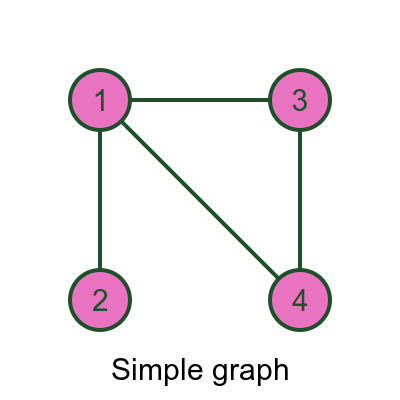
\includegraphics[width=0.3\textwidth]{assets/image/simple-graph.png}
\par}
\vspace{1cm}

\textbf{Dijkstra's algorithm:} là một thuật toán giải quyết bài toán đường đi ngắn nhất từ một đỉnh đến các đỉnh còn lại của đồ thị có hướng không có cạnh mang trọng số không âm. (Nguồn: Wikipedia)

\newpage

\textbf{Các bước thuật toán:}

\begin{enumerate}
   \item \textbf{Khởi tạo:}
   \begin{itemize}[label=\textbullet]
       \item \texttt{dist[start] = 0}, \texttt{dist[other] = $\infty$}
       \item \texttt{parent[all] = -1}
       \item \texttt{visited[all] = false}
   \end{itemize}

   \item \textbf{Priority Queue:} Min-heap chứa các cặp \texttt{(khoảng\_cách, đỉnh)}

   \item \textbf{Vòng lặp chính:}
   \begin{itemize}[label=\textbullet]
       \item Lấy đỉnh \texttt{u} có khoảng cách nhỏ nhất chưa được xử lý
       \item Đánh dấu \texttt{u} đã xử lý
       \item \textbf{Relax} tất cả láng giềng \texttt{v} của \texttt{u}:
       \begin{verbatim}
if dist[u] + weight(u,v) < dist[v]:
   dist[v] = dist[u] + weight(u,v)
   parent[v] = u
   push (dist[v], v) vào priority queue
       \end{verbatim}
   \end{itemize}

   \item \textbf{Kết thúc:} Khi priority queue rỗng
\end{enumerate}

\textbf{Tính chất quan trọng:}
\begin{itemize}[label=\textbullet]
   \item \textbf{Optimal Substructure:} Đường đi ngắn nhất chứa các đường đi con ngắn nhất
   \item \textbf{Greedy Choice:} Lựa chọn tham lam luôn cho kết quả tối ưi
   \item \textbf{Không hoạt động với trọng số âm:} Thuật toán sẽ cho kết quả sai
\end{itemize}

\textbf{Độ phức tạp:}
\begin{itemize}[label=\textbullet]
   \item \textbf{Time Complexity:} O((V + E) log V)
   \begin{itemize}[label=\textendash]
       \item V lần extract-min từ priority queue: O(V log V)
       \item E lần decrease-key: O(E log V)
   \end{itemize}
   \item \textbf{Space Complexity:} O(V)
   \begin{itemize}[label=\textendash]
       \item Mảng \texttt{dist}, \texttt{parent}, \texttt{visited}: O(V)
       \item Priority queue: O(V)
   \end{itemize}
\end{itemize}

\textbf{Cài đặt Python:}
\begin{itemize}[label=\textbullet]
   \item File: \texttt{.\textbackslash code\textbackslash Project\_5\textbackslash BT14\textbackslash dijkstra\_simple\_graph.py}
\end{itemize}

\textbf{Cài đặt C++:}
\begin{itemize}[label=\textbullet]
   \item File: \texttt{.\textbackslash code\textbackslash Project\_5\textbackslash BT14\textbackslash dijkstra\_simple\_graph.cpp}
\end{itemize}
\newpage
\textbf{Format Input (simple\_graph.inp):}
\begin{verbatim}
6 7
0 1 4
1 2 8
2 5 2
0 3 3
3 4 2
4 5 3
1 4 5
\end{verbatim}

\textbf{Giải thích:}
\begin{itemize}[label=\textbullet]
   \item Dòng 1: \texttt{n m} (n = số đỉnh, m = số cạnh)
   \item m dòng tiếp: \texttt{u v w} (cạnh từ đỉnh u đến v với trọng số w)
\end{itemize}

\textbf{Output mẫu:}
\begin{verbatim}
Khoảng cách ngắn nhất từ đỉnh 0:
Đỉnh 0: 0 | Đường đi: 0
Đỉnh 1: 4 | Đường đi: 0 → 1
Đỉnh 2: 12 | Đường đi: 0 → 1 → 2
Đỉnh 3: 3 | Đường đi: 0 → 3
Đỉnh 4: 5 | Đường đi: 0 → 3 → 4
Đỉnh 5: 8 | Đường đi: 0 → 3 → 4 → 5
\end{verbatim}
\newpage
\subsection{Bài toán 15: Thuật toán Dijkstra trên Multigraph}

\begin{problembox}
    \textbf{Let G = (V, E) be a finite multigraph. Implement the Dijkstra's algorithm to find the shortest path problem on G.}
\end{problembox}


\textbf{INPUT:}
\begin{itemize}[label=\textbullet]
    \item Một multigraph G = (V, E) với trọng số không âm
    \item Đỉnh xuất phát (source)
\end{itemize}

\textbf{OUTPUT:}
\begin{itemize}[label=\textbullet]
    \item Khoảng cách ngắn nhất từ đỉnh nguồn đến tất cả các đỉnh khác
    \item Đường đi tương ứng
\end{itemize}

\textbf{Multigraph:} là một đồ thị:
\begin{itemize}[label=\textbullet]
    \item Có nhiều cạnh giữa cùng một cặp đỉnh

\end{itemize}
{\centering
    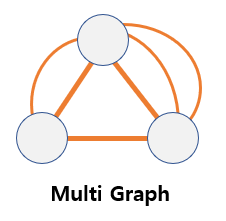
\includegraphics[width=0.3\textwidth]{assets/image/multigraph.png}
\par}
\vspace{1cm}

\textbf{Các bước thuật toán:}

\begin{enumerate}
    \item \textbf{Khởi tạo:}
    \begin{itemize}[label=\textbullet]
        \item \texttt{dist[start] = 0}, \texttt{dist[other] = $\infty$}
        \item \texttt{parent[all] = -1}
        \item \texttt{visited[all] = false}
    \end{itemize}

    \item \textbf{Priority Queue:} Min-heap chứa các cặp \texttt{(khoảng\_cách, đỉnh)}

    \item \textbf{Vòng lặp chính:}
    \begin{itemize}[label=\textbullet]
        \item Lấy đỉnh \texttt{u} có khoảng cách nhỏ nhất chưa được xử lý
        \item Đánh dấu \texttt{u} đã xử lý
        \item Duyệt \textbf{tất cả cạnh} từ \texttt{u} (bao gồm multiple edges)
        \item \textbf{Bỏ qua self-loops:} \texttt{if u == v: continue}
        \item \textbf{Relax} các láng giềng \texttt{v} của \texttt{u}:
        \begin{verbatim}
if dist[u] + weight < dist[v]:
    dist[v] = dist[u] + weight
    parent[v] = u
    push (dist[v], v) vào priority queue
        \end{verbatim}
    \end{itemize}

    \item \textbf{Kết thúc:} Khi priority queue rỗng
\end{enumerate}


\textbf{Cài đặt Python:}
\begin{itemize}[label=\textbullet]
   \item File: \texttt{.\textbackslash code\textbackslash Project\_5\textbackslash BT14\textbackslash dijkstra\_multigraph.py}
\end{itemize}

\textbf{Cài đặt C++:}
\begin{itemize}[label=\textbullet]
   \item File: \texttt{.\textbackslash code\textbackslash Project\_5\textbackslash BT14\textbackslash dijkstra\_multigraph.cpp}
\end{itemize}

\textbf{Format Input (multigraph.inp):}

\begin{verbatim}
6 9
0 1 4
0 1 6
1 2 8
2 5 2
0 3 3
3 4 2
4 5 3
1 4 5
1 4 1
\end{verbatim}

\textbf{Output mẫu:}
\begin{verbatim}
Khoang cach ngan nhat tu dinh 0:
Dinh 0: 0 | Duong di: 0
Dinh 1: 4 | Duong di: 0 -> 1
Dinh 2: 10 | Duong di: 0 -> 3 -> 4 -> 5 -> 2
Dinh 3: 3 | Duong di: 0 -> 3
Dinh 4: 5 | Duong di: 0 -> 3 -> 4
Dinh 5: 8 | Duong di: 0 -> 3 -> 4 -> 5
\end{verbatim}

\newpage

\subsection{Bài toán 16: Thuật toán Dijkstra trên General Graph}

\begin{problembox}
    \textbf{Let G = (V, E) be a general graph. Implement the Dijkstra's algorithm to find the shortest path problem on G.}
\end{problembox}

\textbf{Phân tích bài toán:}

\textbf{INPUT:}
\begin{itemize}[label=\textbullet]
    \item Một general graph G = (V, E)
    \item Đỉnh xuất phát (source)
\end{itemize}

\textbf{OUTPUT:}
\begin{itemize}[label=\textbullet]
    \item Khoảng cách ngắn nhất từ đỉnh nguồn đến tất cả các đỉnh khác
    \item Đường đi tương ứng (nếu thuật toán hoạt động)
\end{itemize}

\textbf{General Graph:} là đồ thị tổng quát nhất, bao gồm:
\begin{itemize}[label=\textbullet]
    \item \textbf{Directed Graph:} Đồ thị có hướng
    \item \textbf{Mixed Graph:} Kết hợp cạnh có hướng và vô hướng
    \item \textbf{Negative Weights:} Có thể có trọng số âm
    \item \textbf{Directed Cycles:} Chu trình có hướng
\end{itemize}

{\centering
    \includegraphics[width=0.8\textwidth]{assets/image/general\_graph.png}
\par}

{\centering
\textbf{General Graph}
\par}
\vspace{1cm}

\textbf {Vấn đề  với General Graph:}

\textbf{Dijkstra's Algorithm KHÔNG hoạt động với trọng số âm} vì:
\begin{itemize}[label=\textbullet]
    \item Greedy choice có thể cho kết quả sai
    \item Một khi đỉnh được đánh dấu "visited", khoảng cách không được cập nhật lại
    \item Trọng số âm có thể tạo ra đường đi ngắn hơn sau khi đỉnh đã được xử lý
\end{itemize}

\textbf{Các bước thuật toán:}

\begin{enumerate}
    \item \textbf{Kiểm tra điều kiện:}
    \begin{itemize}[label=\textbullet]
        \item Duyệt tất cả cạnh trong đồ thị
        \item Nếu phát hiện trọng số âm → dừng thuật toán
        \item Thông báo lỗi và đề xuất Bellman-Ford
    \end{itemize}

    \item \textbf{Khởi tạo (nếu không có trọng số âm):}
    \begin{itemize}[label=\textbullet]
        \item \texttt{dist[start] = 0}, \texttt{dist[other] = $\infty$}
        \item \texttt{parent[all] = -1}
        \item \texttt{visited[all] = false}
    \end{itemize}

    \item \textbf{Priority Queue:} Min-heap chứa các cặp \texttt{(khoảng\_cách, đỉnh)}

    \item \textbf{Vòng lặp chính:}
    \begin{itemize}[label=\textbullet]
        \item Lấy đỉnh \texttt{u} có khoảng cách nhỏ nhất chưa được xử lý
        \item Đánh dấu \texttt{u} đã xử lý
        \item Duyệt \textbf{chỉ cạnh đi ra} từ \texttt{u} (directed)
        \item \textbf{Relax} các láng giềng \texttt{v} của \texttt{u}:
        \begin{verbatim}
if dist[u] + weight < dist[v]:
    dist[v] = dist[u] + weight
    parent[v] = u
    push (dist[v], v) vào priority queue
        \end{verbatim}
    \end{itemize}

    \item \textbf{Kết thúc:} Khi priority queue rỗng
\end{enumerate}

\textbf{Cài đặt Python:}
\begin{itemize}[label=\textbullet]
   \item File: \texttt{.\textbackslash code\textbackslash Project\_5\textbackslash BT14\textbackslash dijkstra\_general\_graph.py}
\end{itemize}

\textbf{Cài đặt C++:}
\begin{itemize}[label=\textbullet]
   \item File: \texttt{.\textbackslash code\textbackslash Project\_5\textbackslash BT14\textbackslash dijkstra\_general\_graph.cpp}
\end{itemize}

\textbf{Format Input:}

\textbf{1. Directed Graph (general\_graph.inp):}
\begin{verbatim}
# directed
6 8
0 1 4
1 2 8
2 5 2
0 3 3
3 4 2
4 5 3
1 4 5
4 1 1
\end{verbatim}

\textbf{2. Graph với trọng số âm (negative\_graph.inp):}
\begin{verbatim}
# directed
4 5
0 1 4
1 2 -3
2 3 2
0 3 7
1 3 5
\end{verbatim}

\textbf{Output mẫu:}

\textbf{1. Directed Graph hợp lệ:}
\begin{verbatim}
Khoảng cách ngắn nhất từ đỉnh 0:
Đỉnh 0: 0 | Đường đi: 0
Đỉnh 1: 4 | Đường đi: 0 → 1
Đỉnh 2: 12 | Đường đi: 0 → 1 → 2
Đỉnh 3: 3 | Đường đi: 0 → 3
Đỉnh 4: 5 | Đường đi: 0 → 3 → 4
Đỉnh 5: 8 | Đường đi: 0 → 3 → 4 → 5
\end{verbatim}

\textbf{2. Graph với trọng số âm:}
\begin{verbatim}
Phát hiện trọng số âm tại cạnh 1→2 (trọng số: -3)
\end{verbatim}

\end{document}